\documentclass[11pt]{article}
\usepackage{mypackages}
\begin{document}

\maketitle

\section{Data}\label{Data}

To train and test our actor-critic and advantage asynchronous actor-critic implementation we will use a framework called OpenAI Gym, which provides an interface to Atari 2600 games, that can be used by developers to compare and test their reinforcement learning algorithms\cite{openAIGym}.

By using OpenAI Gym the information needed for testing our algorithms is easy to collect. 
In the Atari enviroments there is always a finite \textit{action space} and a continous \textit{state space}, where the action space describes the available actions in the environment.

In all environments it's possible to simulate a action in the enviroment. Simulating an action the environment returns a \textit{state}, a \textit{reward} and a \textit{binary signal} which indicate whether the game is done or not.

A state consist of information about the environment, which varies depending on the problem. The reward correspond to what score a real player would have earned.

\subsection{Cart-Pole}

One additional game interface we will be using is made for the Cart-Pole problem.
The game of Cart-Pole consists of balancing a pole connected to the top of a moving cart.
The game ends when the pole is more than 15 degrees from vertical or the cart moves outside of the frame or
the player has reached a score of 200.

\begin{figure}[!h]
    \centering
    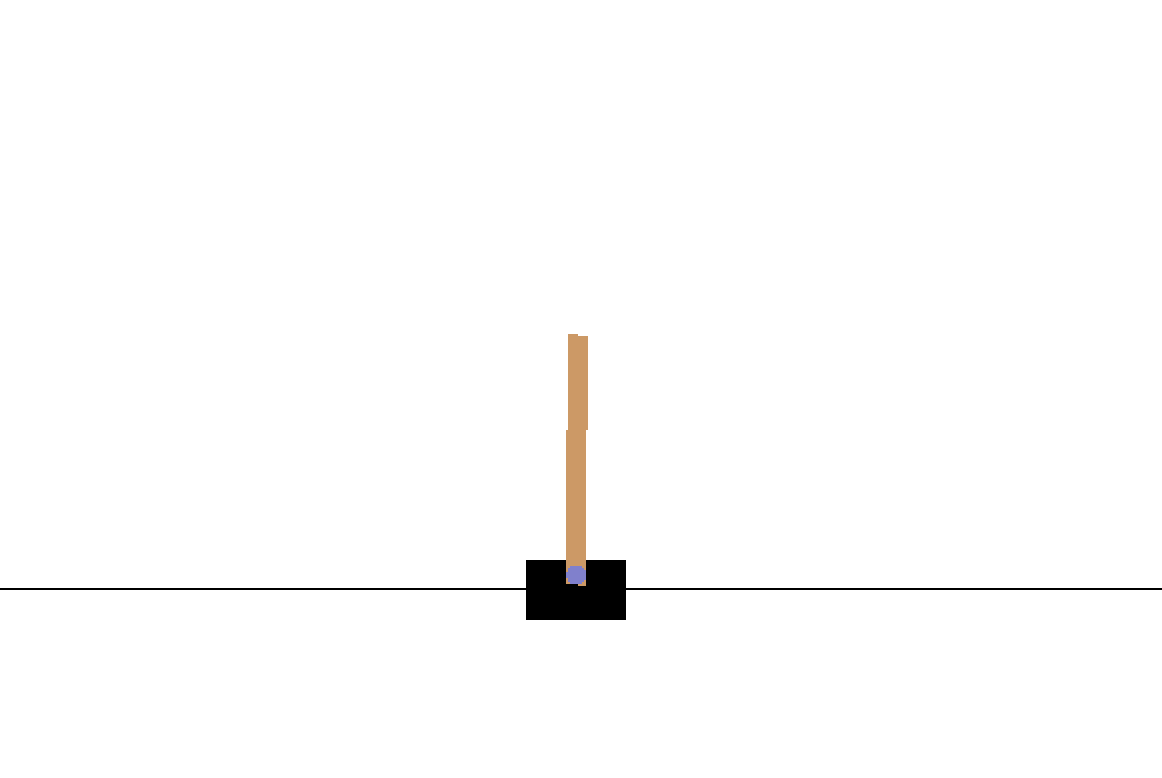
\includegraphics[scale=0.5]{include/cartpole.png}
    \caption{A frame of the Cart-Pole problem.}
    \label{fig:cartpole}
\end{figure}

In the CartPole environment a state consists of four elements: The position of the cart and its velocity, as well as the angle and the angular velocity of the pole.
In the CartPole problem we achieve a reward of +1 for every action performed that does not end the game.
The only available actions are moving left and right, and in our setting the player is not able to choose not to take
an action.

We have chosen the Cart-Pole problem because of its simplicity compared to more advanced games.
An advantage of this problem is that the player is given only relevant information, which means every element
of each state should influence the choice of the next action.

\subsection{Atari 2600}

The real challenge of this project is to improve the model used for playing Cart-Pole to be able to
play Atari 2600 games.
In the OpenAI Gym framework the interface to Atari games resembles the one focused on the Cart-Pole,
with one important difference.
Instead of only being given relevant information about a state, the player is given a frame of the
game in RGB values.
This means that instead of only having 4 items to influence which action to take in a state,
the player is now faced with a frame represented by a 3-dimensional matrix.
All of the games have been normalized to have the same screen size of $210 \times 160$ pixels,
where each pixel contains the three values corresponding to the red, green and blue intensities in the pixel.

In this project we our goal will be to create a generic model that is able to play
any Atari game complying with the structure described above.
However, due to the time limitations of this project we will only
be testing the model on the following games
\begin{itemize}
    \item Pong
    \item ...
\end{itemize}

Upon a more thorough inspection of the Atari environment we have found that
there are pixels in all of the games that never change their RGB value.
These pixels difer from Atari game to Atari game, meaning we can never be sure which part
of the screen we can safely ignore.
In Figure \ref{fig:Atari_env} below we present a single frame from the games
\textit{Pacman}, \textit{Pong}, \textit{Space Invaders} and \textit{Breakout}.
It is easy to spot that each of these games have pixel values that will never change.
E.g. in \textit{Breakout} the gray outer barrier never changes, no matter where the player or ball
is positioned.

\begin{figure}[H]
    \begin{subfigure}[b]{.5\textwidth}
        \centering
        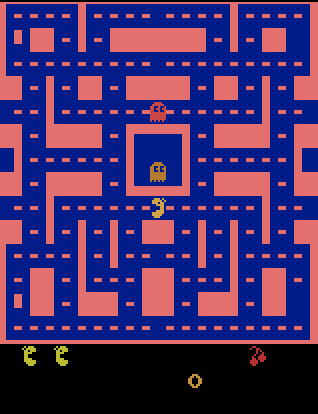
\includegraphics[scale=0.75]{include/pacman.png}
        \caption{A frame from \textit{Pacman}.}
    \end{subfigure}
    \begin{subfigure}[b]{.5\textwidth}
        \centering
        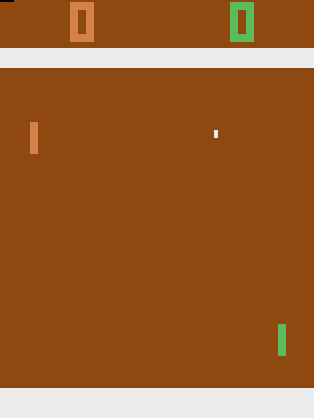
\includegraphics[scale=0.75]{include/pong.png}
        \caption{A frame from \textit{Pong}.}
    \end{subfigure}
    \vskip\baselineskip
    \begin{subfigure}[b]{.5\textwidth}
        \centering
        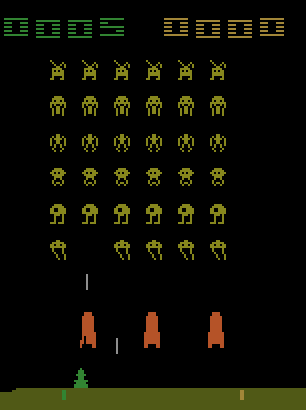
\includegraphics[scale=0.75]{include/space.png}
        \caption{A frame from \textit{Space Invaders}.}
    \end{subfigure}
    \begin{subfigure}[b]{.5\textwidth}
        \centering
        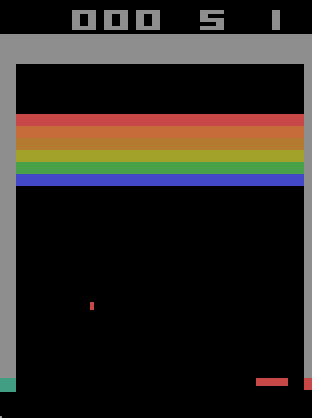
\includegraphics[scale=0.75]{include/breakout.png}
        \caption{A frame from \textit{Breakout}.}
    \end{subfigure}
    \caption{Frames from the \textit{Pacman}, \textit{Pong}, \textit{Space Invaders} and \textit{Breakout} environments}
    \label{fig:Atari_env}
\end{figure}

The main difference between the Cart-Pole problem and the Atari games is that
we will have to extract the features of the environments ourselves.
Since the frames and the available actions vary a lot from game to game
our model will need to train itself on each of the games before it can
be expected to perform properly on each game.

To decrease the workload of the model and increase the pace at which it learns
we will be \textit{grayscaling} the frames.
This will reduce the dimensionality, since each pixel will only have to
store a single value instead of three.

\end{document}
